\documentclass[12pt,a4paper]{jsarticle}
\setlength{\topmargin}{-15mm}
\setlength{\oddsidemargin}{-15mm}
\setlength{\evensidemargin}{-10mm}
\setlength{\textwidth}{180mm}
\setlength{\textheight}{260mm}

\usepackage[top=15truemm,bottom=25truemm,left=20truemm,right=20truemm]{geometry}
\usepackage[latin1]{inputenc}
\usepackage{amsmath}
\usepackage{amsfonts}
\usepackage{amssymb}
\usepackage[dvipdfmx]{graphicx}
\usepackage{listings}
\usepackage{listings,jvlisting}
\usepackage{geometry}

\lstset{
basicstyle={\ttfamily},
identifierstyle={\small},
commentstyle={\smallitshape},
keywordstyle={\small\bfseries},
ndkeywordstyle={\small},
stringstyle={\small\ttfamily},
frame={tb},
breaklines=true,
columns=[l]{fullflexible},
xrightmargin=0zw,
xleftmargin=3zw,
numberstyle={\scriptsize},
stepnumber=1,
numbersep=1zw,
lineskip=-0.5ex
}

\title{}
\author{}
\date{}
\begin{document}
\section*{【使い方】}
\begin{enumerate}
    \item "airfoil\_ajuster.exe"のあるフォルダ内に"original"と"result"の2つのフォルダを作成する。
          \begin{figure}[htbp]
              \begin{center}
                  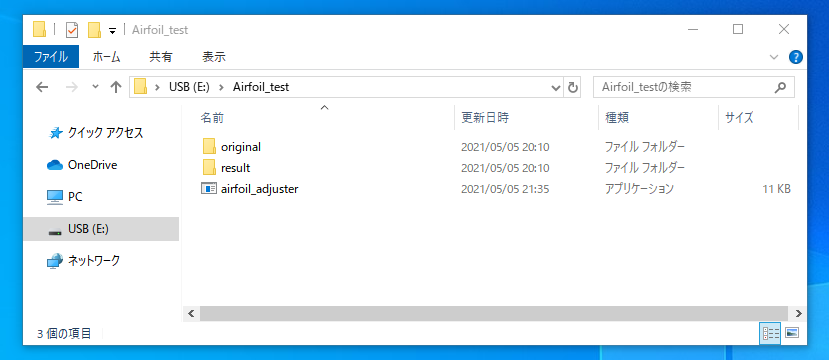
\includegraphics[width=120mm]{gazou_1.png}
              \end{center}
          \end{figure}
    \item "original"のフォルダ内に使用したい翼型の座標を".txt"ファイル形式で保存する。\\
          使用する .txt ファイルの1行目は読み飛ばされることに注意。
          \begin{figure}[htbp]
              \begin{center}
                  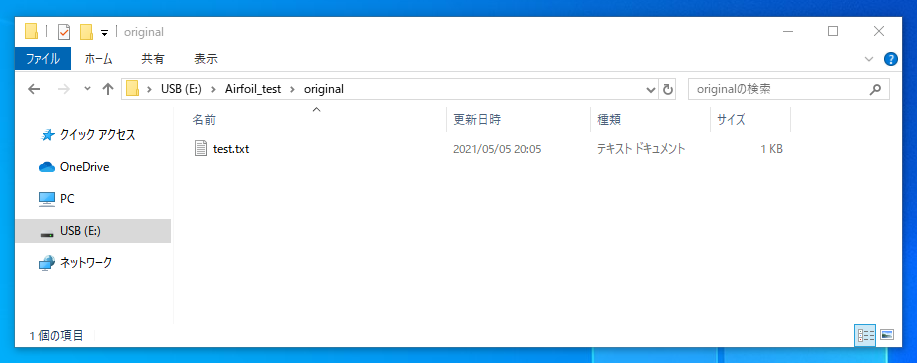
\includegraphics[width=120mm]{gazou_2.png}
              \end{center}
          \end{figure} \\
          \begin{figure}[htbp]
              \begin{center}
                  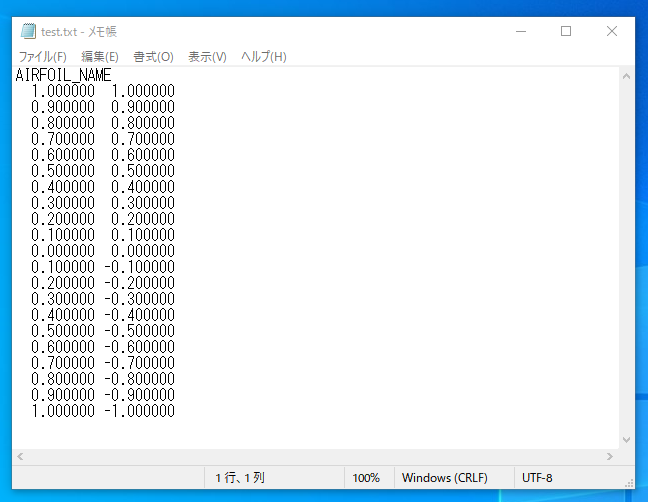
\includegraphics[width=120mm]{gazou_3.png}
              \end{center}
          \end{figure}
          \newpage
    \item "airfoil\_ajuster.exe"をダブルクリックして起動し、翼型のファイル名と任意の翼弦長を入力。\\
          ● このとき、".txt"は入力しなくて良い。    例)"test.txt" を使用する → "test" のみ入力\\
          ● ファイルの読み込みに失敗した場合は、指示にしたがってプログラムを終了し最初からやり直す。\\
          ● 翼弦長は半角で単位は"mm"で入力する。
          \begin{figure}[htbp]
              \begin{center}
                  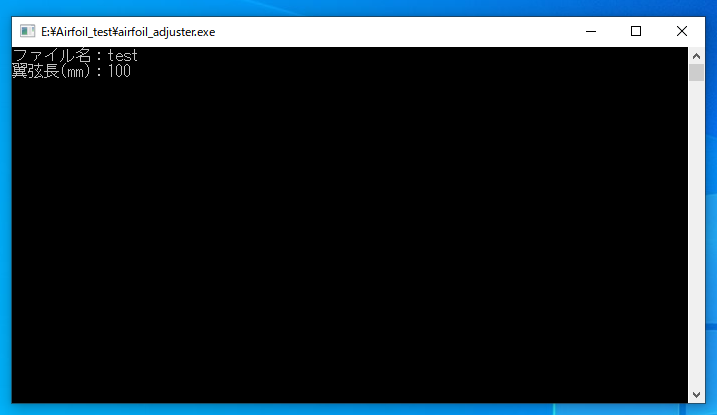
\includegraphics[width=120mm]{gazou_4.png}
              \end{center}
          \end{figure}
    \item プログラムが正常に動作している場合は、以下の画像のように結果が表示される。
          \\確認後、指示にしたがって終了する。\\
          \begin{figure}[htbp]
              \begin{center}
                  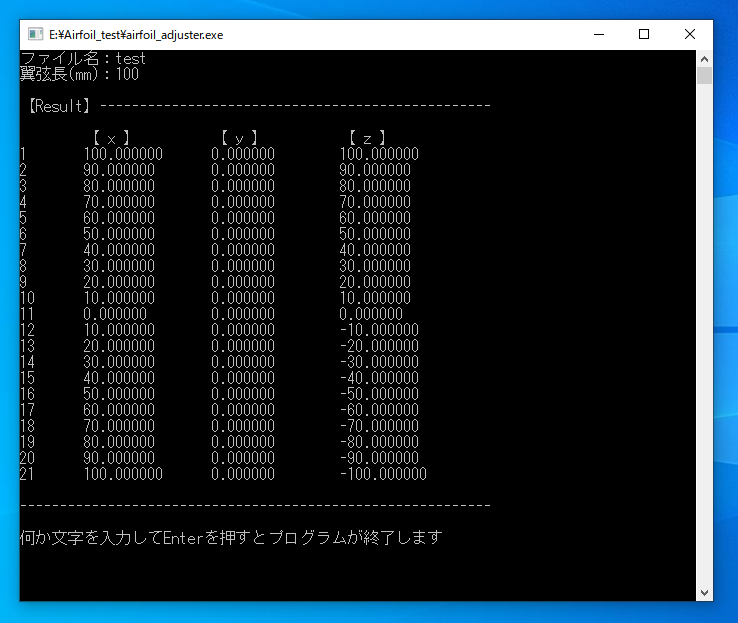
\includegraphics[width=120mm]{gazou_5.png}
              \end{center}
          \end{figure} \\
    \item "result"のフォルダに "ファイル名"\_"翼弦長".csv のファイルで保存される。
\end{enumerate}
\end{document}